      \documentclass[10pt]{article}  

%%%%%%%% PREÁMBULO %%%%%%%%%%%%
\title{Plantilla para prácticas de ESCOM}
\usepackage[spanish]{babel} %Indica que escribiermos en español
\usepackage[utf8]{inputenc} %Indica qué codificación se está usando ISO-8859-1(latin1)  o utf8  
\usepackage{amsmath} % Comandos extras para matemáticas (cajas para ecuaciones,
% etc)
\usepackage{amssymb} % Simbolos matematicos (por lo tanto)
\usepackage{graphicx} % Incluir imágenes en LaTeX
\usepackage{color} % Para colorear texto
\usepackage{subfigure} % subfiguras
\usepackage{float} %Podemos usar el especificador [H] en las figuras para que se
% queden donde queramos
\usepackage{capt-of} % Permite usar etiquetas fuera de elementos flotantes
% (etiquetas de figuras)
\usepackage{sidecap} % Para poner el texto de las imágenes al lado
    \sidecaptionvpos{figure}{c} % Para que el texto se alinie al centro vertical
\usepackage{caption} % Para poder quitar numeracion de figuras
\usepackage{commath} % funcionalidades extras para diferenciales, integrales,
% etc (\od, \dif, etc)
\usepackage{cancel} % para cancelar expresiones (\cancelto{0}{x})
 
\usepackage{anysize}                    % Para personalizar el ancho de  los márgenes
\marginsize{2cm}{2cm}{2cm}{2cm} % Izquierda, derecha, arriba, abajo

\usepackage{appendix}
\renewcommand{\appendixname}{Apéndices}
\renewcommand{\appendixtocname}{Apéndices}
\renewcommand{\appendixpagename}{Apéndices} 

% Para que las referencias sean hipervínculos a las figuras o ecuaciones y
% aparezcan en color
\usepackage[colorlinks=true,plainpages=true,citecolor=blue,linkcolor=blue]{hyperref}
%\usepackage{hyperref} 
% Para agregar encabezado y pie de página
\usepackage{fancyhdr} 
\pagestyle{fancy}
\fancyhf{}
\fancyhead[L]{\footnotesize ESCOM} %encabezado izquierda
\fancyhead[R]{\footnotesize IPN}   % dereecha
\fancyfoot[R]{\footnotesize Propuesta Inicial.}  % Pie derecha
\fancyfoot[C]{\thepage}  % centro
\fancyfoot[L]{\footnotesize Herramienta Para la Planeación de Sostenibilidad Urbana.}  %izquierda
\renewcommand{\footrulewidth}{0.4pt}


\usepackage{listings} % Para usar código fuente
\definecolor{dkgreen}{rgb}{0,0.6,0} % Definimos colores para usar en el código
\definecolor{gray}{rgb}{0.5,0.5,0.5} 
% configuración para el lenguaje que queramos utilizar
\lstset{language=Matlab,
   keywords={break,case,catch,continue,else,elseif,end,for,function,
      global,if,otherwise,persistent,return,switch,try,while},
   basicstyle=\ttfamily,
   keywordstyle=\color{blue},
   commentstyle=\color{red},
   stringstyle=\color{dkgreen},
   numbers=left,
   numberstyle=\tiny\color{gray},
   stepnumber=1,
   numbersep=10pt,
   backgroundcolor=\color{white},
   tabsize=4,
   showspaces=false,
   showstringspaces=false}

\newcommand{\sen}{\operatorname{\sen}}  % Definimos el comando \sen para el seno
%en español

\title{Plantilla para trabajo terminal I de ESCOM}

%%%%%%%% TERMINA PREÁMBULO %%%%%%%%%%%%

\begin{document}

%%%%%%%%%%%%%%%%%%%%%%%%%%%%%%%%%% PORTADA %%%%%%%%%%%%%%%%%%%%%%%%%%%%%%%%%%%%%%%%%%%%
                                                                                    %%%
\begin{center}                                                                      %%%
\newcommand{\HRule}{\rule{\linewidth}{0.5mm}}                                   %%%\left
                                                                                    %%%
\begin{minipage}{0.48\textwidth} \begin{flushleft}

\includegraphics[scale = 0.1]{Imagen/ESCOM-LOGO}
\end{flushleft}\end{minipage}
\begin{minipage}{0.48\textwidth} \begin{flushright}

\includegraphics[scale = 0.35]{Imagen/IPN-LOGO}
\end{flushright}\end{minipage}

                                                                                    %%%
\vspace*{-1.5cm}                                %%%
                                                                                    %%% 
\textsc{\huge Instituto Polit\'ecnico\\ \vspace{5px} Nacional.}\\[1.5cm] 

\textsc{\LARGE Escuela superior de c\'omputo.}\\[1.5cm]                                                   %%%

\begin{minipage}{0.9\textwidth} 
\begin{center}                                                                                  %%%
\textsc{\LARGE Propuesta Inicial}
\end{center}
\end{minipage}\\[0.5cm]
%%%
                                                                                    %%%
            \vspace*{1cm}                                                                       %%%
                                                                                    %%%
\HRule \\[0.4cm]                                                                    %%%
{ \huge \bfseries Herramienta Para la Planeación de Sostenibilidad Urbana.}\\[0.4cm]  %%%
                                                                                    %%%
\HRule \\[1.5cm]                                                                    %%%
                                                                                %%%
                                                                                    %%%
\begin{minipage}{0.46\textwidth}                                                    %%%
\begin{flushleft} \large                                                            %%%
\emph{Autores:}\\ 

Perez Montiel Ulises\\
Sálmean Castro Vicente\\
%%%
            %\vspace*{2cm}  
                                                                %%%
                                                                %%%
\end{flushleft}                                                                     %%%
\end{minipage}      
                                                                %%%
\begin{minipage}{0.52\textwidth}        
\vspace{-0.6cm}                                         %%%
\begin{flushright} \large                                                           %%%
\emph{Asesor:} \\                                                                 %%%
.\\                                             %%%
\end{flushright}                                                                    %%%
\end{minipage}  
\vspace*{1cm}
%\begin{flushleft}
    
%\end{flushleft}
%%%
        \flushleft{\textbf{\Large Proyecto de titulación de Ingeniería en Sistemas Computacionales.} }\\                                                                     %%%
\vspace{2cm}                                                                                
\begin{center}                                                                                  
{\large \today}                                                                 %%%
            \end{center}                                                                        
\end{center}                                                                        
                                                                                    
\newpage                                                                        
%%%%%%%%%%%%%%%%%%%% TERMINA PORTADA %%%%%%%%%%%%%%%%%%%%%%%%%%%%%%%%

\tableofcontents 

\newpage

\section{Resumen.}
Actualmente Megaciudades como la Ciudad de México se encuentran inmersas en una diversidad de problemas por la incapacidad de analizar su complejidad inherente. \\

Uno de los problemas con mayor impacto en la calidad de vida es la movilidad urbana poco sostenible. 

\subsection{Identificación del contexto.}

\begin{figure}[htbp!]
	\begin{center}
		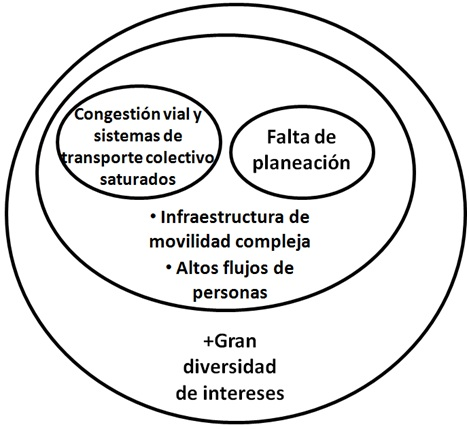
\includegraphics[scale = 0.8]{Imagen/Contexto.jpg}
	\end{center}
\end{figure}

La congestión Vial y los Sistemas de transporte colectivo saturados están correlacionados con la falta de planeación.\\

La infraestructura de movilidad urbana crece y se vuelve mas compleja de analizar con el tiempo.\\

La densidad de población en la ciudad de México es de 6000 habitantes por kilómetro cuadrado lo que da lugar a altos flujos de personas.\\

Existen diversos intereses entre los diferentes niveles de gobierno (Asamblea legislativa y delegaciones), así como de empresas (concesiones en rutas de transporte público, fabricantes de automóviles, constructoras de unidad habitación, comercio, etc).\\

Se analizó esta diversidad de intereses para identificar el problema raíz.\\

\newpage
\subsection{Problema.}

La planeación urbana de la Ciudad de México se lleva en un consejo de desarrollo sostenible, constituido por expertos, especialistas, consultores, académicos y funcionarios, quienes tienen dificultades para comunicar sus ideas y generar valor de los proyectos en la población.\\

Las herramientas existentes son insuficientes para procesar tanta información y predecir los comportamientos emergentes del sistema, se requiere el uso del poder de Cómputo no convencional y la interdisciplina para una toma de decisiones más completa.

\subsection{Análisis del problema.}

Se define al sistema como la infraestructura vial y de transporte con flujos de personas en el mismo.\\
Es un sistema complejo, macroscópico compuesto de sistemas microscópicos que interactúan entre sí con:\\
\begin{itemize}
	\item Propiedades emergentes.
	\item Autoorganización.
	\item Vecindad colectiva.
	\item Evolución y adaptación.
	\item Formación de patrones.
	\item Subsistemas interrelacionados e interdependientes.
	\item Dinámica no lineal.
	\item Decisiones de lógica inteligente. \\
\end{itemize}
	
Se analizó el proceso de toma de decisiones de las personas para encontrar las variables que definen su comportamiento.\\

Se analizó los principales procesos mediante los cuales estas variables se modifican. 

\subsection{Solución propuesta.}
 
Se propone la creación de una herramienta para la planificación de sostenibilidad urbana, dirigida a los expertos y especialistas, que facilite el análisis del sistema complejo, mediante simulaciones enriquecidas con las variables que definen el comportamiento de un individuo, así como los sistemas circundantes que las modifican y las condiciones de los deseos de las personas.  

\subsection{Requerimientos.}
\begin{itemize}
\item  Se requiere optimizar los algoritmos existentes o crear nuevos de tal manera que el sistema simulado sea lo más realista posible

\item Se requiere desarrollar mecanismos para el mejor entendimiento del problema. 

\item Se requiere el apoyo de expertos que nos dirijan en la toma de decisiones, la consideración de requerimientos, y definición del alcance para este proyecto

\end{itemize}
\newpage
\section{Descomposición del problema.}
\begin{figure}[htbp!]
	\begin{center}
		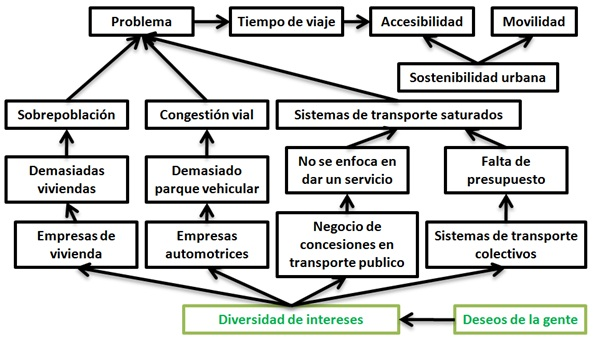
\includegraphics[scale = 1.0]{Imagen/Problema.jpg}
	\end{center}
\end{figure}

El mayor impacto del problema se de como un considerable mayor tiempo de viaje.\\

Debido a los problemas de tráfico, los automovilistas solo en la Ciudad de México tardan 66\% más en llegar a su destino, en comparación con el tiempo que les tomaría cubrir la misma distancia en condiciones ideales de tránsito, indica el estudio, publicado este el 21 de febrero de 2017 y con datos recopilados a los largo de 2016 por TOMTOM TRAFFIC INDEX. \\

El estudio de TomTom explica que los automovilistas tardan hasta 101\% más en llegar a su destino cuando conducen por la tarde, mientras que en la mañana “solo” se tardarían 96\% más del tiempo ideal, en promedio.\\

Así, un conductor en la Ciudad de México pierde en promedio 59 min diaria en el tráfico, lo que da un total de 227 horas de viaje adicionales al ideal por año, establece el estudio.\\

Esto se traduce en una reducción considerable de la accesibilidad al requerir un mayor costo de tiempo y dinero acceder a lugares o personas lejanos, como es el caso de estudiantes y trabajadores que viajan del Estado de México a la Ciudad de México en busca de mejores oportunidades, se pierden en promedio 4 horas al día, lo que da un total de 924 horas al año, 38 días y medio.\\

Para estos últimos, pocos estudios los toman en cuenta, ya que se considera un problema de oportunidades en el Estado de México, no de movilidad.\\

\subsection{La sobrepoblación.}

La gente desea las oportunidades accesibles viviendo en la ciudad, como las escuelas de mayor nivel, empleos mejor pagados, mayor diversidad de personas a quien conocer, mejor preparación en el área de salud, etc.  \\

Las empresas de vivienda siguen satisfaciendo esta necesidad sin tomar en cuenta la sobre demanda de estas mismas oportunidades.  

\subsection{Congestión vial.}

Las empresas siguen invirtiendo en infraestructura en la ciudad para sus operaciones, lo cual genera un incremento considerable en el parque vehicular para este fin. \\

Cada vez mayor cantidad de personas adquieren y hacen uso de un vehículo particular impulsados por la inseguridad, baja calidad de los servicios de transporte público y facilidades de las empresas  automotrices.

\subsection{Sistemas de transporte saturados.}

Las concesiones en transporte público se enfocaron en el  negocio y generan demasiada gente sin posibilidad de ejercer otra actividad con los mismos ingresos, se enfocan en los ingresos y al ser independientes no invierten en mejorar su servicio. \\

Los sistemas de transporte públicos dependientes del gobierno fueron planeados sin tomar en cuenta el abrumador crecimiento de la población, por lo cual dificulta su reestructuración para mejorar sus servicios, además están limitados a  mantener costos bajos y subsidiados para que mayor parte de la población sin ingresos muy altos tenga acceso. 


\subsection{Deseos de la gente.}
Existen proyectos cuyo impacto en la sociedad era positivo y no fue posible realizarlos debido a que la sociedad misma los rechazó oponiéndose.\\

El rechazo se debe mayormente al no considerar las circunstancias locales ó no contar con algún mecanismo que permita a los expertos educar y concientizar a la sociedad acerca del funcionamiento de proyectos contra intuitivos 
\newpage
\section{Definición del sistema.}
El sistema de movilidad:

\begin{itemize}
	\item Forma parte de la estructura vial y de servicios: cuya finalidad es garantizar
	que  las centralidades que conforman la estructura socio económica, espacial; Las
	áreas residenciales, cumplan adecuadamente sus respectivas funciones y se
	garantice de esta forma la funcionalidad de la ciudad.
	\item Debe atender los requerimientos de movilidad de los pasajero y de carga en la zona urbana y área rural así como conectar la ciudad con ciudades vecinas
	\item Integra de manera jerarquizada e interdependiente los modos de transporte de personas y carga con los diferentes tipos de vías y espacios públicos de la ciudad y territorio rural.
	\item Garantiza la movilidad y conexión entre las zonas de servicios y los tejidos residenciales que existen a su alrededor
	 
\end{itemize}

Está conformado por:

\begin{itemize}
\item subsistema vial: vialidades principales, secundarias, locales, rurales, alamedas, pasos peatonales y red de ciclo vialidades.
\item Subsistema de servicios de transporte: Debe responder a los deseos de viaje de la población y a las necesidades de movilización de carga, se constituye de la red de transporte masivo, de corredores troncales de buses y rutas alimentadoras, de transporte publico de otras modalidades, tren de cercanías, transporte público individual, transporte privado, red de estacionamiento publico en vía y fuera de vía de propiedad publica, privada o mixta, terminales de pasajeros de transporte urbano e interurbano, terminales de carga
\item Subsistema de regulación y control: Los centros de control de trafico, red de semaforos y semaforos inteligentes, sistemas tecnológicos de vigilancia y control de operación del tráfico. 

\end{itemize}

\subsection{Propiedades del sistema complejo.}
\begin{itemize}
\item Propiedades emergentes como la paradoja de Braess donde ante la ausencia de grandes vias, con la existencia de una diversidad de caminos alternos surge un comportamiento cooperativo. 
\item Autoorganización: Visto en intersecciones donde no se controla el trafico, los paraderos donde autos y personas se mueven en el mismo espacio, andenes de tren, paradas de transporte publico, etc. 
\item Vecindad colectiva: El comportamiento de cada persona depende en gran medida de lo que suceda en su entorno inmediato.
\item Evolución y adaptación: En accidentes de transito, congestión vial, cierre de vialidades y cualquier otra evento inesperado.
\item Formación de patrones: visto con mayor claridad en condiciones ideales el flujo vehicular tiende a agruparse.
\item Subsistemas interrelacionados e interdependientes al estar integrado por subsistemas y el fraccionamiento de la ciudad 
\item Dinámica no lineal
\item Decisiones de lógica inteligente: mediante el proceso de toma de decisiones ante un evento inesperado \\

\end{itemize}
\subsection{Simplificando la complejidad.}

Encontrando un conjunto de reglas o condiciones simples para cada individuo que interactua con una vecindad es posible recrear comportamientos complejos semejantes a los de sistemas reales. 

\newpage
\section{Proceso de toma de decisiones.}
Para comprender mejor la conducta de las personas, poder definir mejor las reglas requerimos analizar este proceso. \\

\begin{figure}[htbp!]
	\begin{center}
		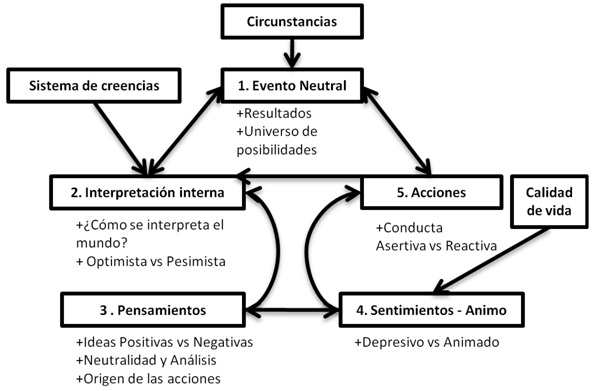
\includegraphics[scale = 1.0]{Imagen/Toma_de_decisiones.jpg}
	\end{center}
\end{figure}

\subsection{ Eventos neutrales.}

Las circunstancias son parte del contexto, del mismo surgen eventos neutrales. Son todos los sucesos que ocurren en el mundo físico, los resultados de nuestras acciones y el contexto en el que nos desarrollamos.

\subsection{ Interpretación interna.}

Los seres humanos interpretamos los eventos neutrales dependiendo de la actitud que tomemos y del sistema de creencias de cada persona, la interpretación interna suele ser inconsciente.\\

Tenemos la capacidad de concientizarnos identificando nuestro sistema de creencias y nuestra actitud.

\subsection{ Pensamientos.}

La interpretación interna sea consciente o inconsciente de originan una serie de pensamientos con una historia consciente, pero una cualidad negativa ó positiva inconsciente. \\

Al concientizarnos de nuestra interpretación podemos elegir la actitud y por ende el sentido de los pensamiento, siendo inclusive neutrales para analizarlo y tomar elecciones  conscientes.

\subsection{ Sentimiento o emoción.}

A la par surgen sentimiento y un estado de ánimo que puede ser Animado mayormente tras pensamiento positivos ó neutrales y una actitud optimista y Depresivo mayor mente tras pensamientos negativo ó neutrales y una actitud pesimista.\\

El estado de ánimo y sentimiento se ven fuertemente influenciado por la calidad de vida, la cual a su vez condiciona las circunstancias. 

\subsection{ Acciones.}

Constituyen la conducta de las personas, la toma final de decisiones, dan origen a los resultados y nuevos eventos.\\

Los pensamientos y el estado de ánimo dan origen a las acciones, siendo esta la respuesta de cada individuo al evento neutral incluyendo el “no tomar ninguna acción” o generando otra interpretación interna.  
\newpage
\section{ Relación con la escasa calidad de vida.}

Una escasa calidad de vida genera un contexto de supervivencia en las circunstancias y el sistema de creencias, los eventos se vuelven adversos para los individuos lo cual  dificulta la consciencia de este proceso de toma de decisiones, generando una conducta reactiva que tiende a retroalimentar el contexto de supervivencia y por consiguiente reducir más la calidad de vida.

\subsection{ Relación con el sistema de creencias.}
\begin{figure}[htbp!]
	\begin{center}
		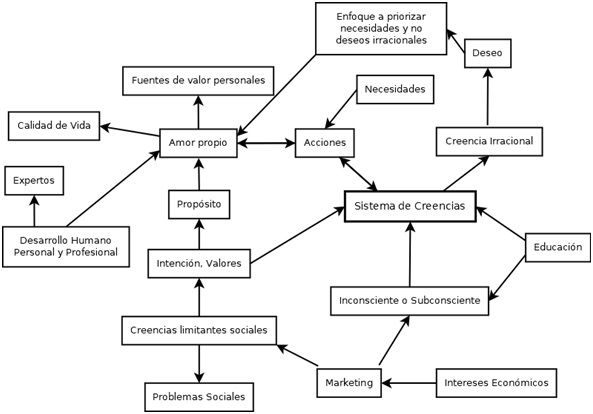
\includegraphics[scale = 1.0]{Imagen/Sistema_de_creencias.jpg}
	\end{center}
\end{figure}

El sistema de creencias juega un papel muy importante al definir el comportamiento de las personas, por ejemplo el proyecto  “El Corredor Cultural Chapultepec” no fue posible implementarse debido a que la sociedad se opuso con base a su sistema de creencias.  \\

Se ve mayormente influenciado por el marketing, la educación y los resultados de las acciones que tomamos día con día. \\

Los intereses Económicos motivados mayormente por deseos irracionales, dan origen al mal uso del Marketing para generar necesidades en las personas, estas al no poder ser satisfechas alimentan los problemas sociales. \\

A su vez el Marketing genera estructuras de comportamiento inconscientes tanto sociales como individuales, dando lugar a una diversidad de creencias.\\

Dichas creencias al ser sociales influyen en los valores y principios de la sociedad, aquellas que son individuales influyen en la imagen personal. \\

Aunque podemos tomar consciencia del mismo, normalmente influye de manera inconsciente en la toma de decisiones, por ejemplo al oponerse a un proyecto cuyo funcionamiento es contra intuitivo.

\section{ Solución propuesta.}
Hoy en día la computación se utiliza para generar conocimiento que de otra forma no estaría a nuestro alcance.  \\

La simulación de flujo vehicular y de personas para planeación de Sistemas de Transporte requiere ser enriquecido con cómputo no convencional al tratarse de un sistema complejo. \\

Se propone crear una herramienta dirigida a los expertos y especialistas para facilitar el análisis del problema mediante simulaciones que tomen en cuenta la complejidad inherente del sistema, así como los sistemas circundantes. \\

\begin{figure}[htbp!]
	\begin{center}
		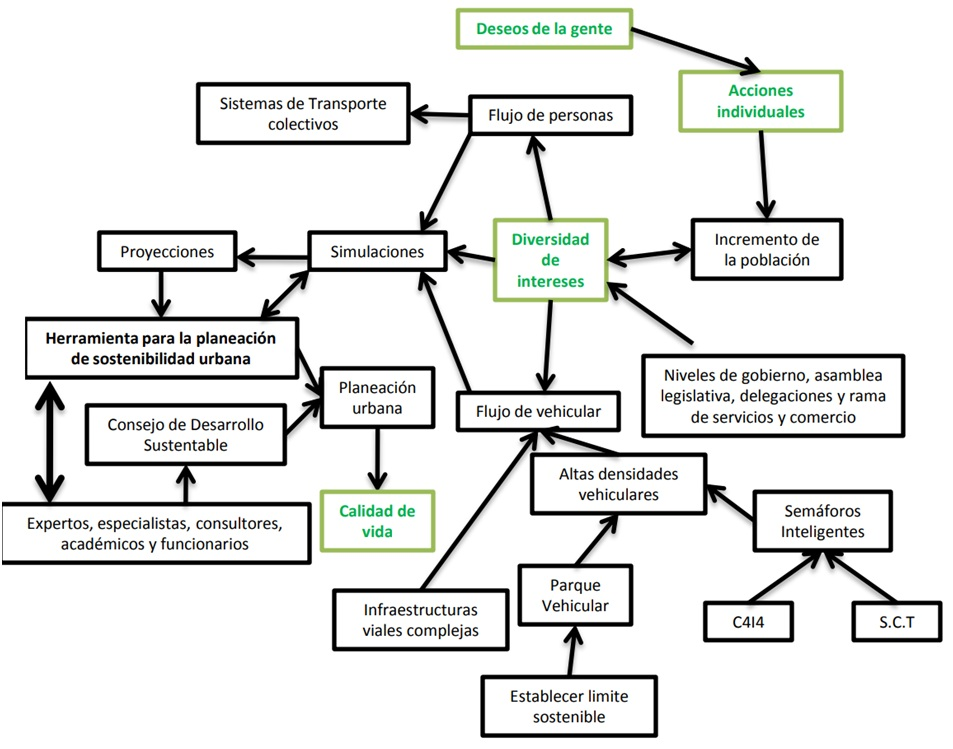
\includegraphics[scale = 0.7]{Imagen/Simulaciones.jpg}
	\end{center}
\end{figure}

\newpage
\subsection{ Resultados esperados.}
Se espera como resultados poder visualizar eventos reales tales como la paradoja de Braess vista en Corea del Sur.\\

Buscar y encontrar reglas sencillas que nos permitan simplificar la complejidad y así ahorrar poder de cómputo. \\

Al ser usada por expertos, mejorar la calidad de vida de los habitantes; Permitiendo la planificación de nuevas estructuras viales, rutas de transporte colectivo como lo son el metrobus, trolebus, mexibus, etc, que optimicen el transporte de pasajeros la movilidad y accesibilidad dentro del Área Metropolitana y la Ciudad de México.\\

Generar mecanismos que permitan mejorar la educación y formulación de leyes que posibiliten un mejor comportamiento cooperativo en la sociedad.   



\end{document}